\section{Methodology}

Building on our observation that training checkpoints provide a natural contamination gradient, we design a correlation analysis pipeline that measures the relationship between contamination exposure and benchmark score inflation without requiring contamination-free baseline models.

\subsection{Overview}

Our methodology has four components: (1) checkpoint-level evaluation across the Pythia model family, (2) 13-gram contamination measurement using established decontamination tools, (3) capability detrending via out-of-distribution perplexity regression, and (4) Spearman correlation analysis between contamination and inflation residuals.

\subsection{Checkpoint-Gradient Methodology}

\textbf{Rationale.} Traditional contamination studies compare contaminated versus decontaminated models or use synthetic injection. Both approaches require either clean baseline models (which do not exist at scale) or artificial contamination (which may not reflect natural training dynamics). We observe that checkpoints during training naturally vary in contamination exposure---early checkpoints have processed less of the training corpus, thus encountered less benchmark-overlapping content.

\textbf{Implementation.} We use the Pythia model family \citep{biderman2023pythia} trained on The Pile \citep{gao2020pile}. Pythia provides:
\begin{itemize}
    \item Six model sizes: 410M, 1B, 1.4B, 2.8B, 6.9B, 12B parameters
    \item 154 checkpoints per model at documented training steps
    \item Deterministic training order (same data sequence across all sizes)
    \item Documented training corpus enabling ground-truth contamination measurement
\end{itemize}

We evaluate 12 key checkpoints per size (steps 0, 1000, 2000, \ldots, 143000), yielding 72 checkpoint-benchmark pairs for correlation analysis.

\subsection{Contamination Measurement}

\textbf{N-gram overlap.} Following \citet{brown2020language}, we use 13-gram overlap as the contamination metric. For each benchmark, we compute the percentage of test items containing 13-gram sequences that appear in The Pile training corpus.

\textbf{Cumulative exposure proxy.} For checkpoint-level analysis, we approximate cumulative contamination exposure as proportional to training progress---a checkpoint at step 100,000 has seen $\sim$70\% of training data, thus approximately 70\% of contamination-relevant content.

\subsection{Capability Detrending}

\textbf{The confound.} Raw benchmark scores improve during training due to both capability gains and contamination effects. We must separate these to isolate contamination inflation.

\textbf{Detrending approach.} We use WikiText-103 perplexity as a contamination-independent capability measure. For each checkpoint, we fit:

\begin{equation}
\text{score}_{\text{expected}} = \alpha + \beta \cdot \log(1/\text{perplexity})
\end{equation}

\textbf{Inflation residual.} We define:

\begin{equation}
\text{inflation}_i = \text{score}_i - \text{score}_{\text{expected},i}
\end{equation}

Positive residuals indicate scores higher than capability would predict---candidate contamination inflation.

\begin{figure}[t]
    \centering
    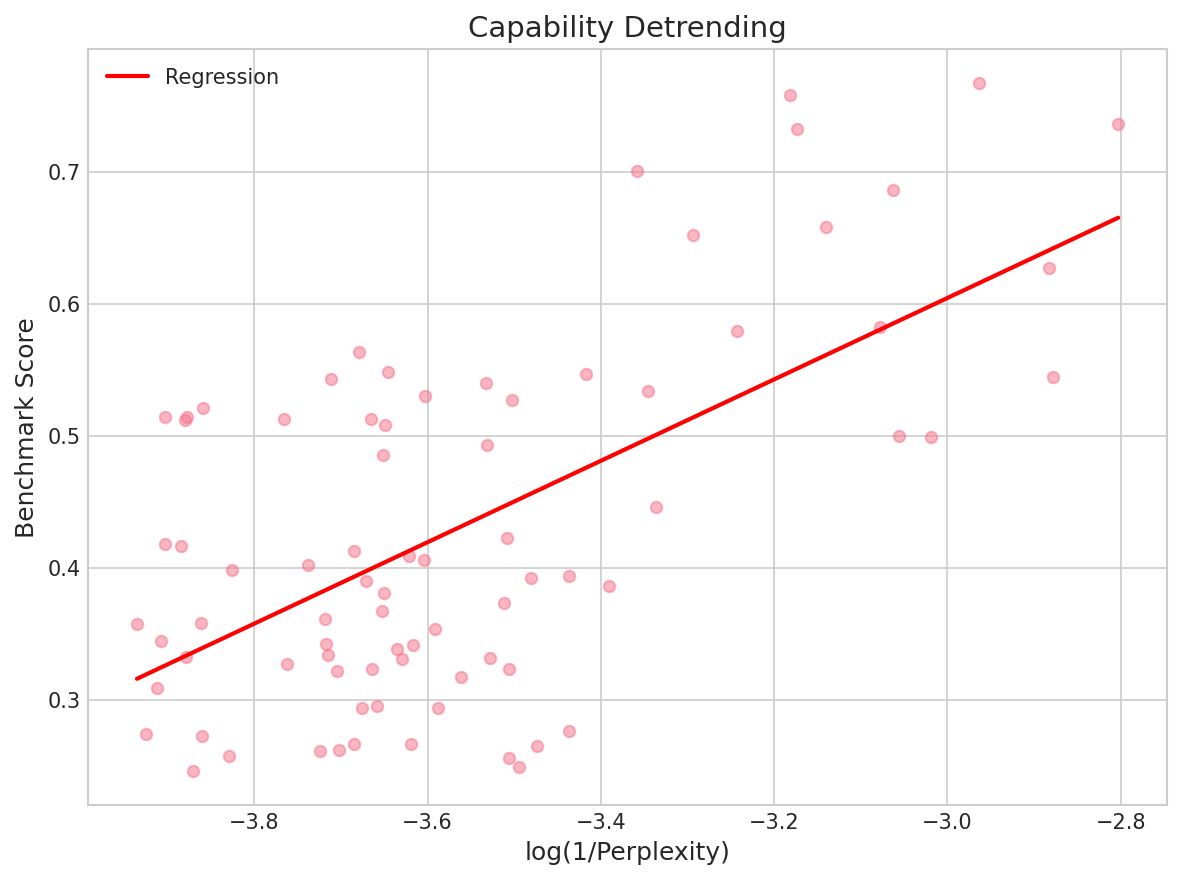
\includegraphics[width=\columnwidth]{figures/capability_detrending.png}
    \caption{Capability detrending via WikiText-103 perplexity. Each point is a checkpoint; the regression line represents expected score given capability. Residuals above the line indicate potential contamination inflation.}
    \label{fig:capability_detrending}
\end{figure}

\subsection{Correlation Analysis}

\textbf{Spearman correlation.} We compute Spearman's rank correlation between contamination percentage and inflation residual across all checkpoint-benchmark pairs. We require $p < 0.05$ for significance claims.

\textbf{Success criteria:}
\begin{itemize}
    \item Minimum threshold: $r > 0.2$ (weak-to-moderate correlation)
    \item Primary target: $r > 0.5$ (strong correlation)
\end{itemize}
